%\documentclass[professionalfonts]{beamer}
\documentclass{beamer}
%\usetheme{Luebeck}
%\usetheme{Copenhagen}
\usetheme{Warsaw}
%\usetheme{Berlin}

\useinnertheme{circles}

%\setbeamertemplate{itemize items}[default]
%\setbeamertemplate{enumerate items}[default]

\usepackage[english]{babel}
\usepackage[utf8]{inputenc}

% AMSLaTeX packages
\usepackage{amsthm}
\usepackage{amsmath}
\usepackage{amsfonts}

\usepackage{xmpmulti}


\usepackage{subfig}
\usepackage{graphicx}

\graphicspath{{../report/}{./}}

\hypersetup{%
	pdftitle={Numerical methods for deforming images},%
	pdfauthor={Robert Crim},%
	pdfsubject={},%
	pdfkeywords={Images, curves, shape registration, image deformation, computational anatomy}%
}


\newcommand{\eq}[1]{(\ref{eq:#1})}
\newcommand{\fig}[1]{Fig. \ref{fig:#1}}
\newcommand{\vect}[1]{\ensuremath{\mathbf{#1}}}
\newcommand{\hvect}[1]{\ensuremath{\hat{\vect{#1}}}}

\newcommand{\pp}[2]{\frac{\partial #1}{\partial #2}}
\newcommand{\vv}[2]{\frac{\delta #1}{\delta #2}}
\newcommand{\angles}[1]{\left\langle #1 \right\rangle}
\newcommand{\eps}{\varepsilon}




\title{Numerical methods for deforming images}
\author[R. Crim]{Robert Crim}
\date[12/9/11]{12 September 2011}
\institute{Imperial College London}

\setcounter{tocdepth}{1}

\begin{document}
\begin{frame}
  \titlepage
\end{frame}

\begin{frame}{Outline}
  \tableofcontents %[part=1,pausesections]
\end{frame}

\section{Introduction}
\subsection{What is computational anatomy?}
\begin{frame}{Computational anatomy}
\begin{block}{What is CA?}
Computational anatomy aims to analyse anatomical shapes \cite{miller2001group, miller2009emerging}  to
determine variability across 
\begin{itemize}
\item populations
\item ages
\item species
\item disease
\end{itemize}
\end{block}

The ability to correlate this variability with other anatomical information may aid in the
early diagnosis of disease \cite{mfca11}.
\end{frame}

\subsection{The problem}
\begin{frame}{Image deformation}
\begin{itemize}
\item The fundamental principle of computational anatomy is that the relative deformation of curves, surfaces, and other objects that take one shape to another may be studied \cite{beg2005computing}.
\vspace{5mm}
\pause
\item There are infinitely many deformations possible, so we are interested in finding the shortest path, or \textbf{geodesic}, between the two shapes.
\end{itemize}
\end{frame}


\begin{frame}{Fluid dynamics analogy}
  \begin{itemize}
  \item Characterise the  deformation as a time-dependent velocity field.
  \item Define as flow which changes one shape to another over a fixed time interval. 
  \item We can express the deformation in terms of kinetic energy
  \end{itemize}

  \pause

  \begin{block}{The problem}
    Finding a velocity field that minimises this energy functional, while ensuring a \textit{template} shape deforms into a \textit{target} shape.
  \end{block}
\end{frame}

\subsection{Inner and outer metrics}
\begin{frame}{Two approaches}

\begin{block}{Outer metrics}
  \begin{itemize}
  \item Used in large deformation diffeomorphic metric matching (LDDMM)
    \cite{grenander1993general,
      beg2005computing,bruveris2011momentum,glaunes2008large}.
  \item   The deforming vector is defined on the entire space.
  \end{itemize}
\end{block}

\begin{exampleblock}{Inner metrics}

\begin{itemize}
\item New approach, first applied to surfaces in \cite{bauer2011new}, developed
  from\cite{michor2005vanishing,michor2003riemannian,younes2008metric}.
\item The deforming vector is defined directly on the image itself.
\end{itemize}

\end{exampleblock}

\end{frame}


\begin{frame}{Inner vs. outer metrics}
\begin{figure}[h!]
  \centering
  \subfloat[Outer  metrics \label{fig:outer_metric}]{
    \includegraphics[width=.35\textwidth]{../misc/outer_field.pdf}}
  \subfloat[Inner metrics \label{fig:outer_metric}]{
    \includegraphics[width=.35\textwidth]{../misc/inner_field.pdf}}
  \caption{Velocity field as defined using outer metrics
    (a), where the vector deforms the entire space, and with inner metrics (b), where the
    deformation occurs directly on the shape itself.}
  \label{fig:metrics}
\end{figure}

\end{frame}

\subsection*{Quick demonstration}
\begin{frame}
\begin{figure}[h!]
  \centering
  \subfloat[Template]{
\includegraphics[width=.5\textwidth]{../cases/ast/qa.pdf}}
  \subfloat[Target]{
\includegraphics[width=.5\textwidth]{../cases/ast/qb.pdf}}
  \label{fig:vectors}
\end{figure}

\end{frame}


\begin{frame}
 \begin{center}
   \multiinclude[format=pdf,graphics={width=0.7\textwidth}]{ast/quiver}
 \end{center}
\end{frame}

\section{Forumulation}

\begin{frame}{Strategy}
  \begin{itemize}
  \item Define a functional $S$
  \item Find the gradient of $S$
  \item Use an optimisation algorithm to find the minimum $S$.
  \end{itemize}
\end{frame}

\subsection{Preliminaries}
\begin{frame}{Curves}
The curves are defined as  continuous periodic functions  $\vect q(s),\, s \in [0,2\pi]$, 
such that $\vect q(0) = \vect q(2\pi)$.
\vspace{5mm}

Given the closed curves $C_{A}$ and $C_B$, the template and target are parameterised  as
\begin{equation}
  \label{eq:qAqB}
  \vect q_{A}(s),\quad \vect q_{B}(s),\quad s \in [0,2\pi]
\end{equation}
\end{frame}

\begin{frame}{Vector field}
A time dependent vector field $\vect u(s,t)$ is applied directly to 
$\vect q(s,t)$, subject to
\begin{equation}
  \vect q_A(s) =\vect q(s,0)   \label{eq:template}
\end{equation}
with the dynamical constraint
\begin{equation}
  \frac{\partial \vect q}{\partial t}(s,t) = \vect u(s,t) ,\quad t \in [0,1] \label{eq:dqdt}
\end{equation}
\end{frame}

\subsection{Constructing the functional}
\begin{frame}{The functional}
  \begin{block}{Requirements}
  We must use functional that
  \begin{itemize}
  \item provides a measure for $\vect u$ (the \textit{metric term})
  \item indicates how close the deformed curve $\vect q(s,1)$ is to the target $\vect q_B$ (the \textit{penalty term})
  \end{itemize}
  \end{block}
  \begin{alertblock}{Note}
    We can't just minimise a norm for $\vect u$ alone. It will always be zero!
  \end{alertblock}
\end{frame}


\begin{frame}{Metric term}
A parameterisation invariant metric is based on the $H^1$ norm, $||f(x)||^2_{H^1} = \int_{\mathbb{R}^2} |f(x)|^2 + |\nabla f(x)|^2\,dx$, is used. It is adapted from a metric used for surfaces in \cite{bauer2011new}.
\begin{equation}
  \label{eq:metric}
  E[\vect u] = \frac{1}{2} \int^{1}_{t=0} \int^{2\pi}_{s=0}\left( \left| \vect u(s,t) \right|^2 
  \left| \frac{\partial \vect q}{\partial s} \right|  + 
  \alpha^2 \frac{ 
    \left| \frac{\partial \vect u}{\partial s}\right|^2}{
    \left| \frac{\partial \vect q}{\partial s}\right|}\right)  \,ds\,dt.
\end{equation}
The constant $\alpha$ is a problem
specific a parameter which controls the characteristic length scale of the
deformations.

\end{frame}


\begin{frame}{Penalty term}
The penalty term is based on the $L^2$ norm
\begin{equation}
  \label{eq:penalty}
  d(\vect q(s,1),\vect q_B) = \frac{1}{2\sigma^2}\int^{2\pi}_{s=0}\left| \vect q(s,1) -
    \vect q_B(s)\right|^2\,ds
\end{equation}
The $\sigma$ constant allows us to control the ``weight'' of the penalty.
\end{frame}



\begin{frame}{The functional $S[\vect u]$}
We combine the metric \eq{metric} and penalty \eq{penalty} terms to
state the optimisation problem

\begin{equation}
  \begin{split}
  \min_{\vect u} S[\vect u] = \frac{1}{2} \int^{1}_{0} \int^{2\pi}_{0}\left| \vect u(s,t) \right|^2 
  \left| \frac{\partial \vect q}{\partial s} \right|  + 
  \alpha^2 \frac{ 
    \left| \frac{\partial \vect u}{\partial s}\right|^2}{
    \left| \frac{\partial \vect q}{\partial s}\right|} \,ds\,dt \\
  +\, \frac{1}{2\sigma^2}\int^{2\pi}_{0}\left| \vect q(s,1) - \vect q_B(s)\right|^2\,ds \label{eq:S}
\end{split}
\end{equation}

\end{frame}

\subsection{The functional derivative}
\begin{frame}{The variational derivative}
The gradient of $S[\vect u]$ can be found starting from its first variation.
\begin{equation}
  \label{eq:lim_dS}
  \int^1_0 \vv{S}{\vect u}\cdot \delta \vect u\,dt = 
  \lim_{\eps \rightarrow 0} \frac{S[\vect u + \eps \delta \vect u] - S[\vect u]}{\eps}
\end{equation}
\end{frame}

\begin{frame}{The variational derivative}
It's difficult to find $\vv{S}{\vect u}$ directly. By temporarily relaxing the constraint \eq{dqdt} and using a Lagrange multiplier and adjoint equation, we can obtain an expression for the gradient
\begin{equation}
  \label{eq:dSdu-deltau}
  \angles{\vv{S}{\vect u}, \delta \vect u} = \angles{\vect u \left|\pp{\vect q}{s}\right|,\delta \vect u} 
  + \alpha^2 \angles{\frac{\pp{\vect u}{s}}{\left|\pp{\vect u}{s}\right|},\pp{}{s}\delta \vect u}
    - \angles{\hvect q,\delta \vect u}
\end{equation}
\end{frame}

% \begin{frame}{The adjoint}
% The adjoint $\hvect q$ is found from
% \begin{equation}
% \begin{split}
%   \label{eq:adjoint}
%   \int^1_0\angles{\hvect q, \delta \pp{}{s} \vect q}\,dt &=  
%   \int^1_0\angles{\frac{d}{dt}\hvect q, \delta \vect q}\,dt -  \int^1_0\angles{\pp{\hvect q}{t}, \delta \vect q }\,dt  \\
%   &= \int^1_0\angles{\frac{d}{dt}\hvect q, \delta \vect q}\,dt - \Big[\angles{\hvect q, \delta \vect q}\Big]^1_0  \\
%   &= \int^1_0\angles{\frac{d}{dt}\hvect q, \delta \vect q}\,dt - \angles{\hvect q\big|_{t=1}, \delta \vect q\big|_{t=0}}
% \end{split}
% \end{equation}
% \end{frame}

\begin{frame}{The adjoint}
The adjoint $\hvect q$ is found from
%We can split the adjoint equation into the weak forms
\begin{equation}
  \label{eq:qh_t1}
  \angles{\delta \vect q, \hvect q\big|_{t=1}} = \frac{1}{\sigma^2}\angles{\delta \vect q, \vect q \big|_{t=1} - \vect q_B}
\end{equation}
\begin{equation}
  \label{eq:dqhdt}
  \angles{\delta \vect q, \pp{\hvect q}{t}} = \angles{\frac{1}{2}\left(\frac{\left|\vect u\right|}{\left|\pp{\vect u}{s}\right|} + \alpha^2\frac{\left|\pp{\vect u}{s}\right|^2}{\left|\pp{\vect u}{s}\right|^3}\right)\pp{}{s}\delta \vect q, \pp{\vect q}{s}}
  \end{equation}
\end{frame}

\section{Implementation}
\subsection{Discretisation}
\begin{frame}{Discretising for $\vect q$}
We first discretise \eq{dqdt} by replacing the derivative with a forward finite
difference
\begin{equation}
  \label{eq:disc_dqdt}
  \pp{\vect q}{t} = \frac{\vect q^{n+1} - \vect q^n}{\Delta t}
\end{equation}

A weak formation is obtained by multiplying by a test function $\vect r$ and
rearranging
\begin{equation}
  \label{eq:disc_q}
  \angles{\vect r, \vect q^{n+1}} = \angles{\vect r, \vect q^n} + \Delta t
    \angles{\vect r, \vect u^n}
\end{equation}

\end{frame}
\begin{frame}{Discretised version of $S[\vect u]$}
We replace with integral with respect to $t$ in \eq{S} with a summation over $N$ time steps.
\begin{equation}
\begin{split}
  \label{eq:S_disc}
  S[\vect u] = \frac{1}{2} \displaystyle \sum_{n=1}^N   \left( 
    \angles{\vect u^n, \vect u^n \left| \pp{\vect q^n}{s} \right|}  + 
  \alpha^2 
  \angles{\pp{\vect u^n}{s}, 
    \frac{\pp{\vect u^n}{s}}{\left|\pp{\vect q^n}{s}\right|}}\right)\\
  + \frac{1}{2\sigma^2}\left\Vert \vect q\big|_{t=1} - \vect q_B\right\Vert^2
\end{split}
\end{equation}
\end{frame}

\begin{frame}{Discretising the adjoint}
The adjoint equation \eq{dqhdt} needs to be discretised
using a backwards finite difference for $\pp{\hvect q}{t}$, since $\hvect
q\big|_{t=1}$ is known from \eq{qh_t1}
\begin{equation}
  \label{eq:disc_dqhdt}
  \pp{\hvect q}{t} = \frac{\hvect q^{n} - \hvect q^{n-1}}{\Delta t}
\end{equation}
Substituting \eq{disc_dqhdt} into \eq{dqhdt}, and using a test function $\hvect
p$, an equation for $\hvect q$ at each time step can be found
\begin{equation}
  \label{eq:disc_qh}
  \angles{\hvect p, \hvect q^{n-1}} = \angles{\hvect p, \hvect q^{n}} - 
  \Delta t\angles{\frac{1}{2}\left(\frac{\left|\vect u^n\right|}{\left|\pp{\vect
            u^n}{s}\right|} + \alpha^2\frac{\left|\pp{\vect
            u^n}{s}\right|^2}{\left|\pp{\vect u^n}{s}\right|^3}\right)\pp{\hvect p}{s}, \pp{\vect q^n}{s}}
  \end{equation}
\end{frame}

\begin{frame}{Discretising the gradient}
Finally, \eq{dSdu-deltau} is solved in terms of a test function $\vect v$ at
each time step
\begin{equation}
  \label{eq:dSdu}
  \angles{\vv{S}{\vect u^n}, \vect v} = \angles{\vect u^n \left|\pp{\vect q^n}{s}\right|, \vect v} 
  + \alpha^2 \angles{\frac{\pp{\vect u^n}{s}}{\left|\pp{\vect u^n}{s}\right|},\pp{}{s}\vect v}
    - \angles{\hvect q^n,\vect v}
\end{equation}
\end{frame}

\subsection{Finite elements}
\begin{frame}{Finite elements with FEniCS}

\begin{itemize}
\item FEM is  handled by Python libraries from the FEniCS project \cite{logg2007fenics}.
\item Second order Lagrange elements are used on an interval $0 \leq s \leq 2\pi$, though the scheme works with higher orders.
\end{itemize}

\begin{block}{FEniCS benefits}
  \begin{itemize}
    \item The weak form equations are expressed similar to mathematical notation.
    \item Much of the problem formulation is automated.
    \item  JIT compiler to used to compile equations into highly optimised C code  \cite{logg2007automated}.
    \end{itemize}
\end{block}

\end{frame}

\subsection{Optimisation algorithm}
\begin{frame}{BFGS-L}
The code uses the limited memory Broyden--Fletcher--Goldfarb-- Shanno (L-BFGS) \cite{byrd1995limited} algorithm to compute the minimal $S[\vect u]$.

\begin{itemize}
\item BFGS, like all optimisation algorithms, is iterative. 
\item Starts with an initial guess, and successively improves on an estimated solution.
\item Stops when a specified convergence tolerance is
reached, or at a max iteration count.
\end{itemize}

BFGS is a quasi-newton method, meaning the Hessian matrix $\nabla^2 f(x)$ is approximated.

\end{frame}



\subsection{Procedure overview}
\begin{frame}{Procedure overview}
At each iteration of the optimiser, the code calculates the values of $S[\vect u]$ and $\vv{S}{\vect u}$ using the steps
\begin{enumerate}
\item Populate array of $\vect q$ at each time step using \eq{disc_q}.
\item Calculate $S$ using \eq{S_disc}.
\item Find $\hvect q|_{t=1}$ from \eq{qh_t1}.
\item Populate array of $\hvect q$ at each time step using \eq{disc_qh}.
\item Solve for $\vv{S}{\vect u}$ with \eq{dSdu} at each time step.
\end{enumerate}
\end{frame}

\subsection{Verification}
\begin{frame}{Test results}
The error should approach zero as $\eps \rightarrow 0$
\begin{equation}
  \label{eq:error_o1}
  E_1 = \left| \displaystyle \sum^{N}_{t=0} \angles{\vv{S}{\vect u},\vect v}\Delta
    t - \lim_{\eps \rightarrow 0} 
  \frac{S[\vect u + \eps \vect v] - S[\vect u]}{\eps} \right|
\end{equation}

We can also formulate a second order equation for the error as
\begin{equation}
  \label{eq:test_2nd}
   E_2 = \left\vert \displaystyle \sum^{N}_{t=0} \angles{\vv{S}{\vect u},\vect v}\Delta t - \lim_{\eps \rightarrow 0} 
  \frac{S[\vect u + \eps \vect v] - S[\vect u - \eps \vect v] }{2\eps} \right\vert
\end{equation}
\end{frame}

\begin{frame}
\begin{figure}[h!]
  \centering
  \includegraphics[width=0.8\textwidth]{img/convergence.pdf}
  \caption{Test using first and second order approximation of
    \eq{lim_dS} }
  \label{fig:convergence}
\end{figure}


\end{frame}

\section{Numerical experiments}
\subsection{Large deformation with curves and corners}
\begin{frame}{Self intersection of the curve}
\begin{figure}
  \centering
  \subfloat{\includegraphics[width=0.25\textwidth]{../cases/numbers/step_0.pdf}}
  %\subfloat{\includegraphics[width=0.333\textwidth]{../cases/numbers/step_1.pdf}}
  \subfloat{\includegraphics[width=0.25\textwidth]{../cases/numbers/step_2.pdf}}
  \subfloat{\includegraphics[width=0.25\textwidth]{../cases/numbers/step_3.pdf}}\\
  %\subfloat{\includegraphics[width=0.333\textwidth]{../cases/numbers/step_4.pdf}}
  \subfloat{\includegraphics[width=0.25\textwidth]{../cases/numbers/step_5.pdf}}
  \subfloat{\includegraphics[width=0.25\textwidth]{../cases/numbers/step_6.pdf}}
  %\subfloat{\includegraphics[width=0.333\textwidth]{../cases/numbers/step_7.pdf}}
  \subfloat{\includegraphics[width=0.25\textwidth]{../cases/numbers/step_8.pdf}} 
\label{fig:intersection}
\end{figure}
\end{frame}

\subsection{Parmeterisation dependence}
\begin{frame}{Reparameterisation of the target}
\begin{figure}
  \centering
  \subfloat{\includegraphics[width=0.20\textwidth]{../reparams/path_0.pdf}}
  \subfloat{\includegraphics[width=0.20\textwidth]{../reparams/path_1.pdf}}
  \subfloat{\includegraphics[width=0.20\textwidth]{../reparams/path_2.pdf}}
  \subfloat{\includegraphics[width=0.20\textwidth]{../reparams/path_3.pdf}}\\
  \subfloat{\includegraphics[width=0.20\textwidth]{../reparams/steps_0.pdf}}
  \subfloat{\includegraphics[width=0.20\textwidth]{../reparams/steps_1.pdf}}
  \subfloat{\includegraphics[width=0.20\textwidth]{../reparams/steps_2.pdf}}
  \subfloat{\includegraphics[width=0.20\textwidth]{../reparams/steps_3.pdf}}\\
  \caption{Changes in path and shape evolution for reparameterisations of the
    same target shape. The top row shows the path taken by a selection of points,
    the bottom row shows the evolution of the shape at 10 time steps.}
  \label{fig:reparams}
\end{figure}

\end{frame}


\begin{frame}{Average between shapes}
\begin{figure}[h!]
  \centering
  \subfloat{
\includegraphics[width=0.333\textwidth]{../cases/people/qa.pdf}}
  \subfloat{\includegraphics[width=0.333\textwidth]{../cases/people/q_5.pdf}}
  \subfloat{
\includegraphics[width=0.333\textwidth]{../cases/people/qb.pdf}}
  %\subfloat{\includegraphics[width=0.333\textwidth]{../cases/people/quiver_0.pdf}}
  %\subfloat{\includegraphics[width=0.333\textwidth]{../cases/people/quiver_5.pdf}}
  %\subfloat{\includegraphics[width=0.333\textwidth]{../cases/people/quiver_9.pdf}}
  \caption{Shapes at $t=0$, $t=0.5$, and $t=1$, with the middle shape
    showing the average between the template and target.}
\label{fig:average}
\end{figure}  
\end{frame}

\subsection{Shape classification}
\begin{frame}{Identification of shape}

\begin{block}{Can we identify this shape?}
\begin{figure}
  \centering
  
\includegraphics[width=0.25\textwidth]{img/shapematch/test_star.png}
\end{figure}
\end{block}
From this library of known shapes?
\begin{figure}
  \centering
  \subfloat{
\includegraphics[width=.12\textwidth]{img/shapematch/circle.png}}\,
  \subfloat{
\includegraphics[width=.12\textwidth]{img/shapematch/hexagon.png}}
  \subfloat{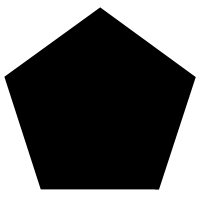
\includegraphics[width=.12\textwidth]{img/shapematch/pentagon.png}}
  \subfloat{
\includegraphics[width=.12\textwidth]{img/shapematch/square.png}}
  \subfloat{
\includegraphics[width=.12\textwidth]{img/shapematch/star.png}}
  \subfloat{
\includegraphics[width=.12\textwidth]{img/shapematch/star_11.png}}
  \subfloat{
\includegraphics[width=.12\textwidth]{img/shapematch/star_six.png}}
  \subfloat{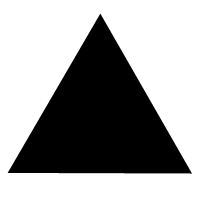
\includegraphics[width=.12\textwidth]{img/shapematch/triangle.png}}
\end{figure}

\end{frame}

\begin{frame}{Yes!}
\begin{figure}[h!]
  \centering
  \subfloat[$S = 8.92$]{
\includegraphics[width=.25\textwidth]{img/shapematch/circle.pdf}}
  \subfloat[$S = 14.30$]{
\includegraphics[width=.25\textwidth]{img/shapematch/hexagon.pdf}}
  \subfloat[$S = 6.05$]{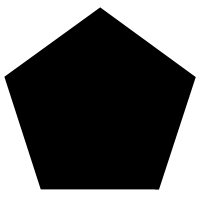
\includegraphics[width=.25\textwidth]{img/shapematch/pentagon.pdf}}
  \subfloat[$S = 23.84$]{
\includegraphics[width=.25\textwidth]{img/shapematch/square.pdf}}\\
  \subfloat[Match: $S = 1$]{
\includegraphics[width=.25\textwidth]{img/shapematch/star.pdf}}
  \subfloat[$S = 8.93$]{
\includegraphics[width=.25\textwidth]{img/shapematch/star_11.pdf}}
  \subfloat[$S = 12.31$]{
\includegraphics[width=.25\textwidth]{img/shapematch/star_six.pdf}}
  \subfloat[$S = 16.48$]{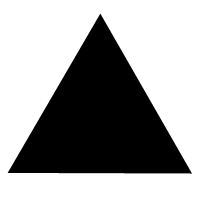
\includegraphics[width=.25\textwidth]{img/shapematch/triangle.pdf}}
  %\caption{Evolution of shape at each timestep for each respective shape in the
  %  library. Normalised with the lowest value of $S$}
  \label{fig:shape_match}
\end{figure}
\end{frame}

\begin{frame}{Font classification}
A more difficult problem is the classification between serif and sans-serif fonts.

\begin{figure}[h!]
  \centering
  \includegraphics[width=0.5\textwidth]{img/serifs.pdf}
  \caption{Left side shows a serif font with serifs circled in red. Sans-serif font is on the right.}
\end{figure}
\end{frame}


\begin{frame}{Success}
\begin{figure}[h!]
  \centering
  \subfloat[Helvetica $\rightarrow$ Arial]{\includegraphics[width=0.5\textwidth]{img/helvetica/sans-arial.pdf}}
  \subfloat[Helvetica  $\rightarrow$ Times]{\includegraphics[width=0.5\textwidth]{img/helvetica/serif-times.pdf}}
  \caption{Helvetica is successfully classified as a \textbf{sans-serif} font.}
\end{figure}

\end{frame}

\begin{frame}{Failure}
\begin{figure}[h!]
  \centering
  \subfloat[Times  $\rightarrow$ Arial]{\includegraphics[width=0.5\textwidth]{img/times/sans-arial.pdf}}
  \subfloat[Times  $\rightarrow$ Sabon]{\includegraphics[width=0.5\textwidth]{img/times/serif-sabon.pdf}}
\caption{Times is inaccurately classified as a \textbf{serif} font.}
\end{figure}

\end{frame}

\section{Conclusion}
\subsection{Outlook and suggestions}
\begin{frame}{Outlook}

The results suggest this approach is promising and warrants further investigation.
\vspace{5mm}
\begin{block}{Limitations}
\begin{itemize}
\item The parameterisation dependence of the penalty term.
\item No automatic calibration of $\sigma$.
\item Resource intensive solution method.
\end{itemize}
\end{block}
\end{frame}

\begin{frame}{Further work}
\begin{itemize}
\item Reparameterise the curves at the start, so the penalty term is parameterisation invariant \cite{clark2011reparam}.
\vspace{10mm}
\item Use inner metrics with a geodesic shooting method.
\end{itemize}
\end{frame}

\subsection*{Questions}
\begin{frame}

\begin{figure}
\subfloat{\includegraphics[width=0.2\textwidth]{../cases/thanks/qa.pdf}}
\subfloat{\includegraphics[width=0.2\textwidth]{../cases/thanks/q_1.pdf}}
\subfloat{\includegraphics[width=0.2\textwidth]{../cases/thanks/q_2.pdf}}
\subfloat{\includegraphics[width=0.2\textwidth]{../cases/thanks/q_3.pdf}}
\subfloat{\includegraphics[width=0.2\textwidth]{../cases/thanks/q_4.pdf}}
\end{figure}
\centering
\Huge{Any questions?}

\begin{figure}
\subfloat{\includegraphics[width=0.2\textwidth]{../cases/thanks/q_5.pdf}}
\subfloat{\includegraphics[width=0.2\textwidth]{../cases/thanks/q_6.pdf}}
\subfloat{\includegraphics[width=0.2\textwidth]{../cases/thanks/q_7.pdf}}
\subfloat{\includegraphics[width=0.2\textwidth]{../cases/thanks/q_8.pdf}}
\subfloat{\includegraphics[width=0.2\textwidth]{../cases/thanks/q_9.pdf}}
\end{figure}

\end{frame}

\begin{frame}[allowframebreaks]{References}
\bibliographystyle{unsrt}
\bibliography{../report/refs.bib}
\end{frame}

\end{document}